\begin{frame}{Conceptos básicos}
	\begin{itemize}
      	\item ¿Qué es un ataque a un sistema informático?
      	\item Tipos de ataque más comunes.
    		\item TCP/IP.
    \end{itemize}
      
    	\begin{figure}[H]
	    \centering
	    \hbox{
	    \begin{minipage}[b]{0.45\textwidth}
	    		\centering
		    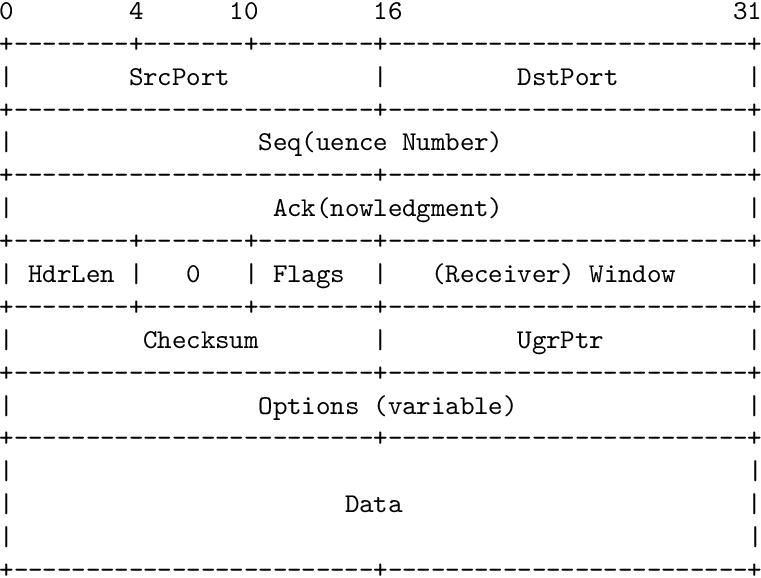
\includegraphics[width=\linewidth]{../Memoria/img/ent-problema/SegmentoTCP.png}
		    \caption{Esquema segmento TCP \cite{tcpsegment}.}
		    \label{fig:SegmentoTCP}
	    \end{minipage}
	    
	    \hspace{1cm}
	        
	    \begin{minipage}[b]{0.45\textwidth}
		    \centering
		    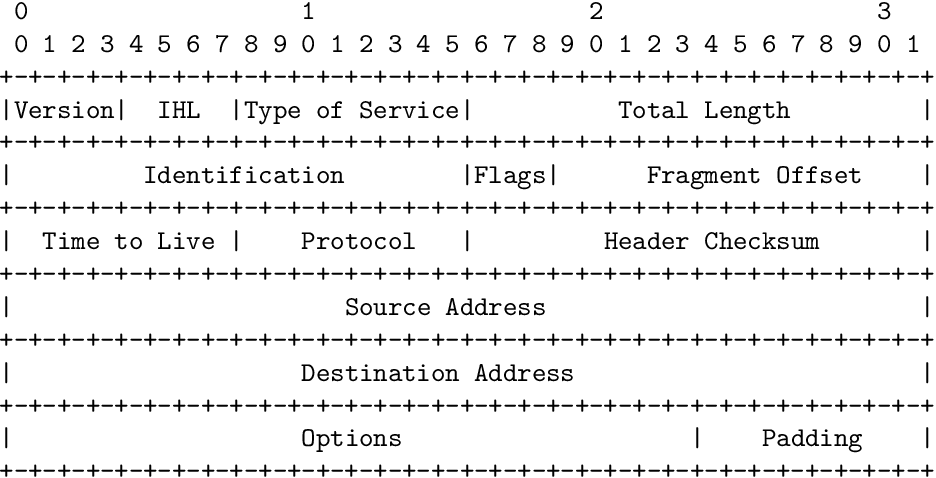
\includegraphics[width=\linewidth]{../Memoria/img/ent-problema/PaqueteIP.png}
		    \caption{Formato de la cabecera IPv4 \cite{paqueteip}.}
		    \label{fig:PaqueteIP}
	    \end{minipage}	
	    }
	\end{figure}
	
\end{frame}

\begin{frame}{Prueba}
	\begin{itemize}
		\item Importancia de protegerse frente a un ataque informático.
		\item Importancia de detectar rápidamente frente a un ataque informático.
	\end{itemize}
\end{frame}

\begin{frame}{Soluciones actuales}
	\begin{itemize}
		\item Cortafuegos de próxima generación (NGFW).
		\item Sistema de detección de intrusiones (IDS).
		\item Sistema de prevención de intrusiones (IPS).
	\end{itemize}
\end{frame}
